%! TEX rootmain.tex

\chapter{Piano}

The piano combines a percussive excitation mechanism with a large resonant structure. A key press triggers a sequence of mechanical events that culminates in string vibration, energy transfer through the bridge, and sound radiation by the soundboard. Following the course outline, the discussion starts from the instrument anatomy and then moves to the piano action, strings and hammers, the role of the soundboard, sound decay, and finally tuning and inharmonicity.

\section{Anatomy of the Instrument}

A simplified scheme of the piano highlights four main subsystems: the keyboard and action, the strings, the soundboard, and the structural frame. Their interaction determines both the mechanical response and the acoustic output. A simplified block diagram of the piano highlights the main coupled subsystems, as shown in figure \ref{fig:piano_simplified_scheme}.

\begin{figure}[!htb]
\centering
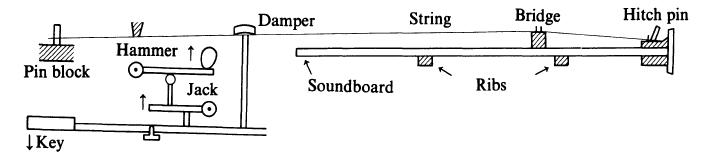
\includegraphics[width=0.9\linewidth]{00_Images/02_chapter/img37.jpg}
\caption{Simplified scheme of the piano as coupled subsystems from key to soundboard}
\label{fig:piano_simplified_scheme}
\end{figure}

\subsection{From Key Press to Soundboard Vibration}

When a key is depressed, the sound production chain can be described as a sequence of coupled events. In compact form, the process is the following:

\begin{itemize}
    \item The damper is raised, allowing the string to vibrate.
    \item The action throws the hammer against the strings.
    \item The strings are set into vibration.
    \item The string vibration is transmitted to the soundboard through the bridge.
\end{itemize}

Each step has been progressively refined in historical development, because small improvements in the action and in the structural design strongly affect controllability, repeatability, and tonal result.

\subsection{Strings Layout in a Grand Concert}

A grand concert piano contains a large number of strings, with geometrical and material variations across the compass. Typical figures are as follows:

\begin{itemize}
    \item The total number of strings is about 243, with lengths ranging from about \SI{2}{\meter} in the bass to about \SI{5}{\centi\meter} in the treble.
    \item 68 notes are produced by triplets of unwrapped strings.
    \item 7 notes are produced by three wrapped strings.
    \item 5 notes are produced by pairs of wrapped strings.
    \item 8 notes are produced by single strings wrapped with one or two layers of wire.
\end{itemize}

A relevant construction detail is that bass strings overlap middle strings in order to locate their action closer to the center of the soundboard. A representative layout of strings and soundboard in a grand concert is shown in figure \ref{fig:grand_strings_layout}.

\begin{figure}[!htb]
\centering
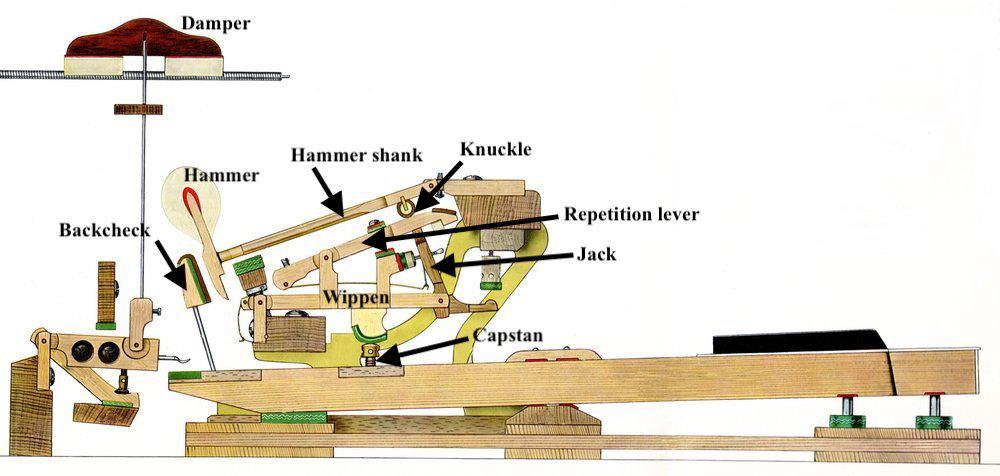
\includegraphics[width=0.8\linewidth]{00_Images/02_chapter/img43.jpg}
\caption{Typical strings layout and soundboard arrangement in a grand concert piano}
\label{fig:grand_strings_layout}
\end{figure}

\subsection{Soundboard and Frame}

The soundboard is typically made from spruce, with thickness up to about \SI{1}{\centi\meter} and grain running along the length of the piano. Ribs beneath the board stiffen it in the cross-grain direction. Besides its radiating role, the soundboard assembly has an important static function, because the total string tension can be very large. In a grand piano the overall force may exceed \SI{20}{\tonne}, and robust cast-iron frames are required to withstand the load while maintaining tuning stability.

\subsection{Upright Piano Variants and Striking Mechanism}

Upright pianos may vary considerably in design, mainly because the striking mechanism differs from the grand. The hammer motion is horizontal, so the return of parts to their rest position depends on springs. Three representative arrangements are commonly distinguished:

\begin{itemize}
    \item In a full-size upright, the striking mechanism is located above the keys and connected to them through sticks.
    \item In a studio upright, the action is mounted directly over the keys, without sticks.
    \item In a small spinet, the action is below the keys, and drop sticks transmit the key motion to the action.
\end{itemize}

Common upright variants and their main geometric differences are compared in figure \ref{fig:upright_variants}.

\begin{figure}[!htb]
\centering
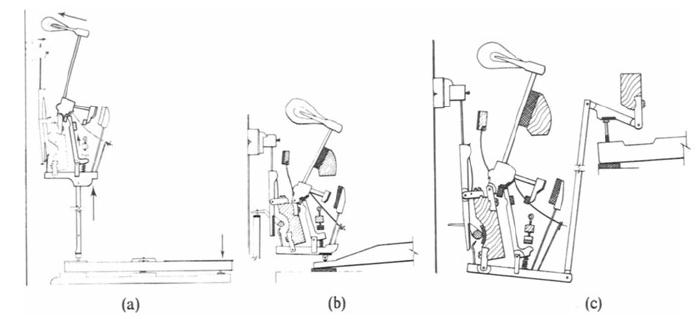
\includegraphics[width=0.8\linewidth]{00_Images/02_chapter/img58.jpg}
\caption{Examples of upright piano variants and corresponding construction differences}
\label{fig:upright_variants}
\end{figure}

\section{Piano Action}

\subsection{Kinematic Sequence During a Keystroke}

When a key is pressed down, the piano action converts the finger force into a fast hammer motion through a sequence of constrained movements and releases. The main stages can be summarized as follows:

\begin{itemize}
    \item The wippen, jack, and hammer are raised.
    \item The key begins to raise the damper, freeing the string.
    \item The jack engages the regulator and rotates away from the knuckle.
    \item After impact, the hammer rebounds and is caught by the backcheck, while the knuckle depresses the repetition lever.
    \item If the key is released slightly, the backcheck releases the hammer and the repetition lever lifts it until the jack returns below the knuckle, enabling repetition.
\end{itemize}

The main phases of the action motion during a keystroke are summarized in figure \ref{fig:piano_action_sequence}.

\begin{figure}[!htb]
\centering
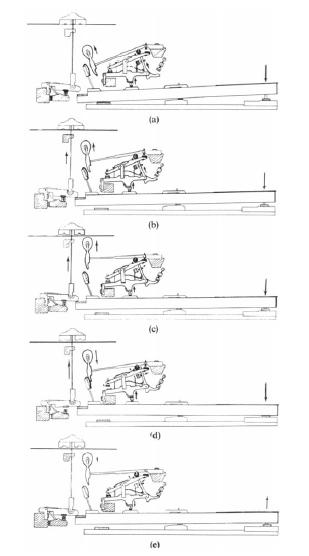
\includegraphics[width=0.7\linewidth]{00_Images/02_chapter/img85.jpg}
\caption{Kinematic sequence of the piano action during a keystroke}
\label{fig:piano_action_sequence}
\end{figure}

\subsection{Simplified Lever Model}

To connect the player input to the mechanical outcome, a simplified diagram models the action as two levers transmitting a key depression force \( F \) applied at the touch point \( P \). During the acceleration phase, the touch point moves with velocity \( v_p(t) \), while the hammer velocity is \( v_h(t) \). A typical effective velocity ratio is approximately constant for most of the touch, and then the hammer swings free. A simplified lever representation of the action is shown in figure \ref{fig:simplified_lever_model}.

\begin{figure}[!htb]
\centering
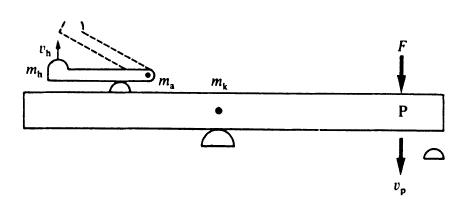
\includegraphics[width=0.6\linewidth]{00_Images/02_chapter/img117.jpg}
\caption{Simplified lever model relating key motion, contact point, and hammer motion}
\label{fig:simplified_lever_model}
\end{figure}

\subsection{Equation of Motion and Touch Acceleration}

During about \SI{70}{\percent} of the touch, the velocity ratio is approximately
\[
\frac{v_h}{v_p} = 5.5
\]
The static force needed to raise the key is about
\[
F_s = \SI{0.44}{\newton}
\]
which is equivalent to raising a mass of about \SI{45}{\gram}. In addition to \( F_s \), the applied force must accelerate the moving parts of the key and action. With \( m_k \) the effective key mass, \( m_a \) the equivalent mass of other action parts, \( m_h \) the hammer mass, and \( a_p \) the acceleration at the touch point, the equation of motion is written as
\[
F - F_s = m_k(0.018a_p) + m_a(0.72a_p) + m_h(5.5a_p)
\]
By substituting typical numerical values, the touch acceleration becomes
\[
a_p = \frac{dv_p}{dt} = 3.3(F-\SI{0.44}{\newton})
\]

\subsection{Key Travel Time and Hammer Striking Velocity}

If the depressing force is assumed constant over the key travel, the time \( T_s \) needed to move through a distance \( s \) to the stop is
\[
T_s = \sqrt{\frac{2s}{a_p}}
\]
For a typical travel \( s=\SI{9}{\milli\meter} \), this yields
\[
T_s = 0.074\sqrt{(F-\SI{0.44}{\newton})}
\]
The hammer striking velocity \( V_0 \) follows from the velocity ratio during the constrained phase,
\[
V_0 = 5.5a_pT_s = 1.34\sqrt{(F-\SI{0.44}{\newton})}
\]
A plot of \( V_0 \) and \( T_s \) as a function of \( F \) shows that increasing force produces a larger striking velocity and a shorter key depression time, with indicative regions corresponding to dynamic levels from \( pp \) to \( ff \). The dependence of striking velocity and travel time on applied force is illustrated in figure \ref{fig:striking_velocity_travel_time}.

\begin{figure}[!htb]
\centering
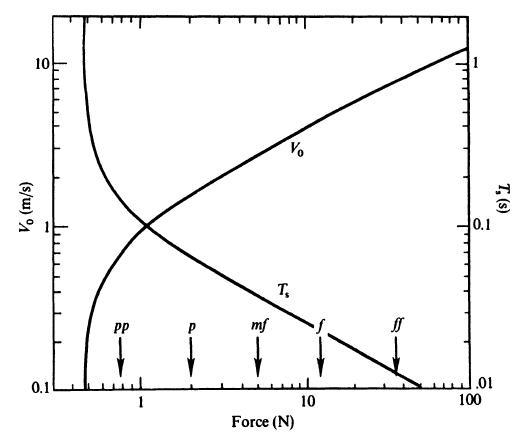
\includegraphics[width=0.6\linewidth]{00_Images/02_chapter/img132.jpg}
\caption{Hammer striking velocity and key travel time versus applied force}
\label{fig:striking_velocity_travel_time}
\end{figure}

\subsection{Non-constant Force Profiles and Timing Control}

If the applied force is not constant in time, the same striking velocity, and therefore a comparable impact strength on the strings, can be obtained with different key depressing times. Skilled players can exploit this by controlling timing within a chord, making one note sound slightly earlier or later than the others while maintaining similar intensity.

\subsection{Pedals and Their Functions}

Pianos typically have two or three pedals, modifying sustain and excitation conditions.

\begin{itemize}
    \item The right pedal is the sustaining pedal and lifts the dampers, so struck strings continue vibrating after the keys are released.
    \item The left pedal differs between grand and upright designs. In most grands it shifts the action sideways so that treble hammers strike two strings instead of three, called the una corda pedal. In many uprights, and in some grands, it moves the hammers closer to the strings, reducing travel and striking force, often called the soft pedal.
    \item The third pedal may act as a sostenuto pedal, sustaining only notes already depressed when the pedal is engaged. In some instruments it lifts only bass dampers, while in some uprights it functions as a practice pedal by inserting felt between hammers and strings to mute the tone.
\end{itemize}

\section{Piano Strings}

Strings have the fundamental task of capturing the energy brought by the hammer, converting it into vibrational energy, storing it in their normal modes, and transmitting this energy to the bridge and soundboard.

\subsection{Materials, Tension, and Construction} 

Piano strings are high-strength steel wires. In order to produce tones with the expected loudness, high tensions are used: the tensile stress is around
\[
\sigma \approx \SI{1000}{\newton\per\milli\meter\squared}
\]
For steel, this corresponds to an elongation of about
\[
\varepsilon \approx \SI{0.5}{\percent}
\]
Treble strings are solid wire, while lower strings are wound with copper wire. The winding diameter varies widely across the compass, from about twice the core diameter for the lowest string to about one fourth for the highest wrapped string. The winding is mainly used to increase mass per unit length while minimizing bending stiffness. Strings are clamped on one side and pinned on the other, so the normal modes are expected to lie between those of clamped-clamped and pinned-pinned stiff strings. In practice, expressions for pinned stiff strings are commonly used as a workable approximation. Typical trends of tension and inharmonicity along the keyboard are summarized in figure \ref{fig:string_scales_trends}.

\begin{figure}[!htb]
\centering
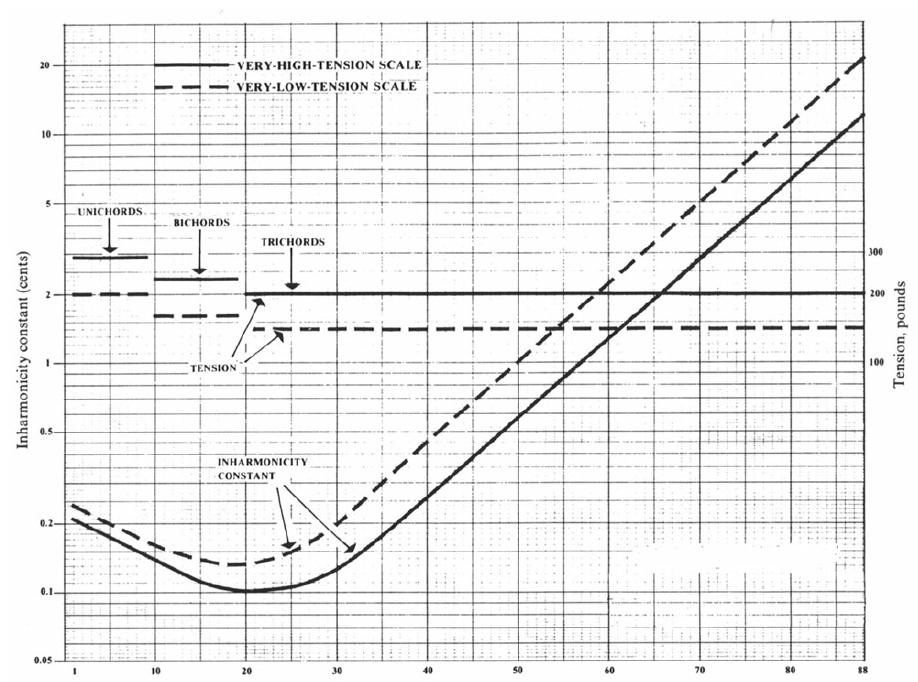
\includegraphics[width=0.6\linewidth]{00_Images/02_chapter/img147.jpg}
\caption{Typical string-scale trends along the keyboard: tension and inharmonicity evolution}
\label{fig:string_scales_trends}
\end{figure}

\subsection{Stiff-string Partials and Inharmonicity} 

For a pinned stiff string, the \( n \)-th partial can be expressed as
\[
f_n = n f_1 \left[\frac{1+n^{2}B}{1+B}\right]^{1/2}
\]
where \( B \) is the inharmonicity coefficient. A representative value for piano strings is
\[
B = 0.0004
\]
With this value, the \( 17 \)-th partial is shifted by about one partial position, namely close to the frequency of the \( 18 \)-th partial of an ideal flexible string. The inharmonicity can be expressed in cents as
\[
I_n = 1200\log_2\left[1+n^{2}B\right]^{1/2} \approx 866\,n^{2}B = b n^{2}
\]
where
\[
b = 866 B
\]

\subsection{Variation Along the Scale} 

Piano string scales show a systematic variation of tension and inharmonicity with note number. The reported trend highlights that different design choices (for instance very-high-tension versus very-low-tension scales) lead to different inharmonicity levels across the keyboard, while keeping the overall musical compass.

\subsection{Transmission-line Representation} 

Strings can be modeled by electrical transmission lines. Mass and compliance per unit length are represented by inductance and capacitance per unit length, respectively, while the transverse displacement is represented by current. In this analogy, the hammer can be represented by an inductance with a voltage across its terminals, and different switch configurations describe the contact condition between hammer and string. A transmission-line representation of the string and its coupling to excitation/termination is shown in figure \ref{fig:string_transmission_line_model}.

\begin{figure}[!htb]
\centering
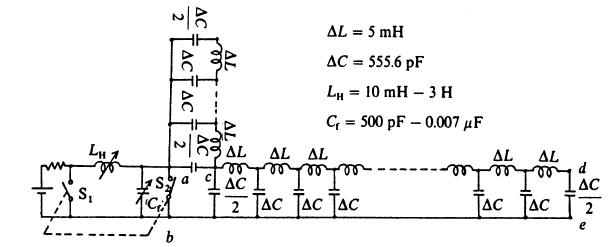
\includegraphics[width=0.8\linewidth]{00_Images/02_chapter/img162.jpg}
\caption{Transmission-line model of the string with excitation and termination elements}
\label{fig:string_transmission_line_model}
\end{figure}

\section{Piano Hammers}

Piano hammers are typically made of a hardwood core covered by one or two layers of felt. Modern bass hammers are larger than treble ones, so typical hammer masses range from about \SI{10}{\gram} in the bass down to about \SI{3.8}{\gram} in the treble. The felt covering is a key element in determining the tone.

\begin{itemize}
    \item The thickness of the outer felt layer increases from treble to bass, and its density is typically in the range
    \[
    \rho_f \in \SIrange{0.6}{0.7}{\gram\per\centi\meter\cubed}
    \]
    \item Hard hammers tend to produce a brilliant but potentially harsh sound, while soft hammers produce a duller tone.
\end{itemize}

A crucial point is that felt does not behave as a linear spring. Instead of Hooke's law, a nonlinear relation is used,
\[
F = K \xi^{p}
\]
where \( \xi \) is the compression. For used hammers, the exponent is typically in the range
\[
p \in \SIrange{2.2}{3.5}{}
\]
while for unused hammers it is often smaller,
\[
p \in \SIrange{1.5}{2.8}{}
\]
Moreover, \( K \) and \( p \) may differ between compression and relaxation, resulting in hysteresis. An important consequence of this nonlinearity is that the felt is effectively harder at high impact velocity than at low velocity, which contributes to a brighter sound at stronger dynamics. The striking point and the hammer mass influence the spectral envelope of the excited string motion. If an idealized hammer strikes the string at a fraction \( \beta \) of the string length, harmonics for which the striking point coincides with a node are strongly attenuated. This is consistent with the standard dependence of harmonic amplitudes on the factor \( \sin(n\pi\beta) \), which vanishes when \( n\beta \) is an integer. If the hammer mass is not negligible compared to the string mass, the spectrum shows a progressively stronger high-frequency roll-off above a certain partial number. For heavier hammers, the hammer may remain in contact with the string long enough for several reflected pulses to return, attenuating the motion and reducing clarity. Computer simulations indicate that, for a hard hammer, the high-frequency energy spectrum envelope can exhibit an approximate slope of \SI{-6}{\decibel} per octave. For treble strings, where the hammer mass can exceed the string mass, the slope may reach about \SI{-12}{\decibel} per octave. Experimental waveforms illustrate that hammer-string contact time must be interpreted relative to the fundamental period, and that reflections from the agraffe may appear as distinct features in the measured string velocity. Representative waveforms and spectra for different registers, together with typical contact-time values, are shown in figure \ref{fig:waveforms_spectra_contact_time}.

\begin{figure}[!htb]
\centering
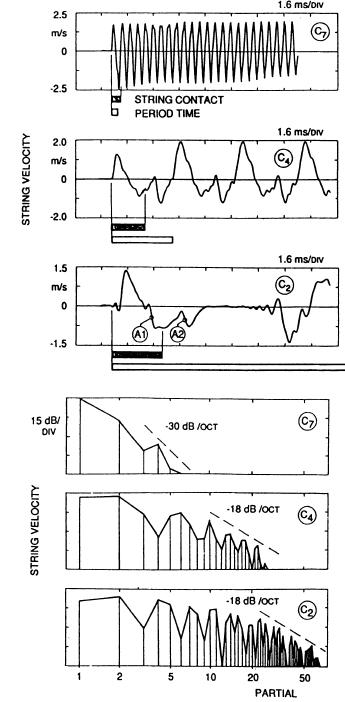
\includegraphics[width=0.6\linewidth]{00_Images/02_chapter/img190.jpg}
\caption{Waveforms and spectra for different registers and corresponding contact-time indications}
\label{fig:waveforms_spectra_contact_time}
\end{figure}

\subsection{Voicing}

Voicing is the set of operations used to adjust hammer hardness, its gradient, and related properties in order to obtain a desired tone. Typical interventions are the following:

\begin{itemize}
    \item If the hammer is too soft, it can be hardened by removing soft felt or by chemical hardening processes.
    \item If the hammer is too hard, it can be softened by piercing the felt with needles.
\end{itemize}

Voicing is typically applied differently depending on the desired dynamic range, with distinct regions of the hammer surface associated with loud, medium, and soft playing. The qualitative effect of hammer voicing on tone color is summarized in figure \ref{fig:hammer_voicing} and the influence of hammer hardness on the radiated spectrum is illustrated in figure \ref{fig:hammer_hardness_spectra}.

\begin{figure}[!htb]
\centering
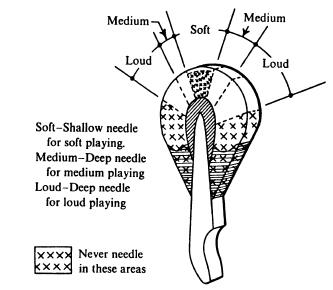
\includegraphics[width=0.6\linewidth]{00_Images/02_chapter/img204.jpg}
\caption{Hammer voicing and its influence on spectral balance across playing levels}
\label{fig:hammer_voicing}
\end{figure}

\begin{figure}[!htb]
\centering
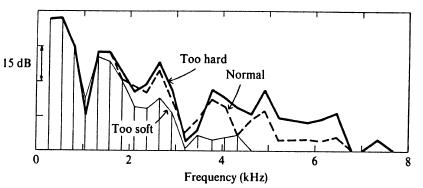
\includegraphics[width=0.7\linewidth]{00_Images/02_chapter/img223.jpg}
\caption{Effect of hammer hardness on the spectrum for a representative note}
\label{fig:hammer_hardness_spectra}
\end{figure}

\subsection{Striking Point Ratio}

Let \( d \) be the distance between the agraffe and the hammer contact point, and \( L \) the total string length. The ratio \( d/L \) is a relevant design parameter. In modern pianos, the ratio \( d/L \) is more constant along the keyboard than in older instruments. The choice of striking point reflects a compromise between fundamental strength and tone quality.

\begin{itemize}
    \item Reducing \( d/L \) tends to make the sound thinner because the fundamental becomes weaker.
    \item Too large a ratio can reduce clarity because the hammer dwell time becomes excessive.
\end{itemize}

Typical striking-point ratios along the keyboard, and their historical evolution, are shown in figure \ref{fig:striking_point_ratio}.

\begin{figure}[!htb]
\centering
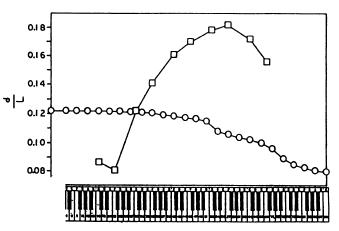
\includegraphics[width=0.7\linewidth]{00_Images/02_chapter/img238.jpg}
\caption{Striking point ratio along the keyboard for historical and modern designs}
\label{fig:striking_point_ratio}
\end{figure}

\section{Sound Board}

The soundboard of the piano is made of glued strips of spruce. Under the board, ribs run in the cross-grain direction: their main role is to stiffen the soundboard across the grain, bringing the cross-grain stiffness closer to the along-grain one. The soundboard has two distinct functions:

\begin{itemize}
    \item A static function: it must bear the load transferred from strings and bridges, typically between \SI{900}{\newton} and \SI{1800}{\newton}.
    \item An acoustic function: it is the main radiating component of the instrument and it converts vibrational energy coming from bridges and strings into acoustic energy.
\end{itemize}

Modern pianos have two bridges, a main (treble) bridge and a bass bridge. The bass bridge is typically \SIrange{2}{3}{\centi\meter} taller than the treble bridge, so that bass strings can pass over the treble ones. Bridges act as impedance transformers: they present to the strings an input impedance much higher than the one that would be obtained if strings were attached directly to the soundboard. Moreover, bridges enable the soundboard to respond to string vibration both normal to the board and in the plane of the board, including contributions associated with longitudinal string motion.

\subsection{Treble and Bass Bridges}

The relative placement of bass and treble bridges is arranged to accommodate overlapping string groups and to drive the soundboard over a large region, rather than concentrating excitation close to one edge. The treble and bass bridges and their placement on the soundboard are shown in figure \ref{fig:treble_bass_bridges}.

\begin{figure}[!htb]
\centering
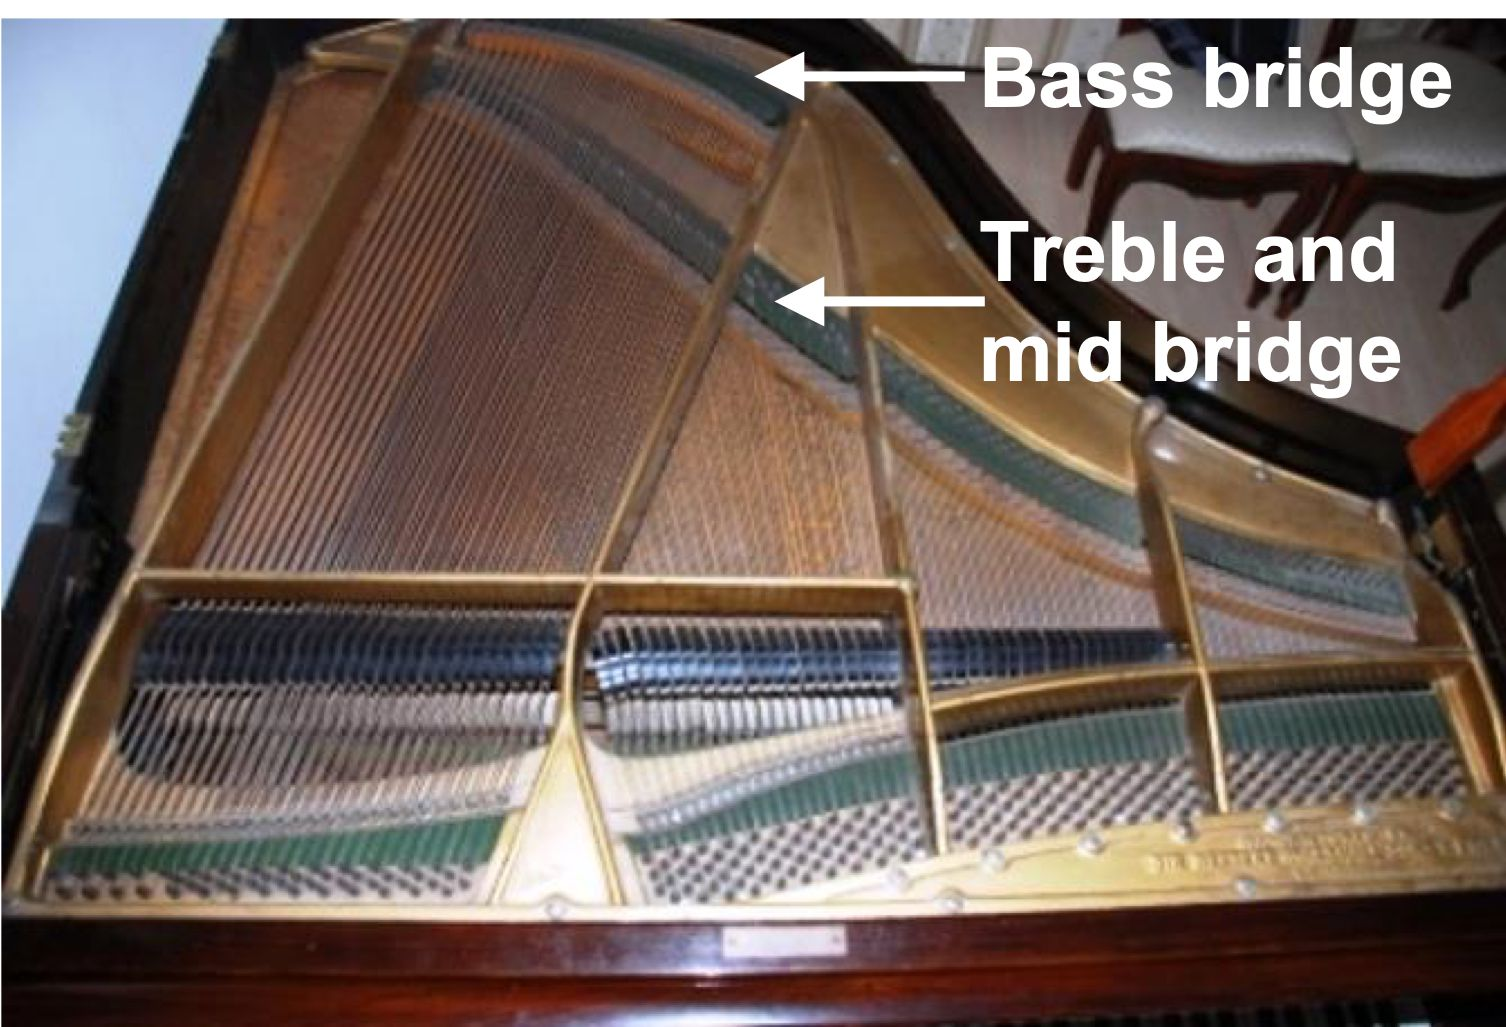
\includegraphics[width=0.7\linewidth]{00_Images/02_chapter/img249.jpg}
\caption{Treble and bass bridges on the piano soundboard}
\label{fig:treble_bass_bridges}
\end{figure}

\subsection{Cantilevered Bridges}

In small pianos, bridges may be cantilevered to shift the soundboard driving point away from the stiff perimeter zone while still allowing the longest possible string lengths. The cantilever region separates the string-bridge attachment point from the bridge-board attachment point, so that the board is driven more effectively in its vibratory area. A schematic representation of cantilevered bridge solutions is shown in figure \ref{fig:cantilevered_bridges}.

\begin{figure}[!htb]
\centering
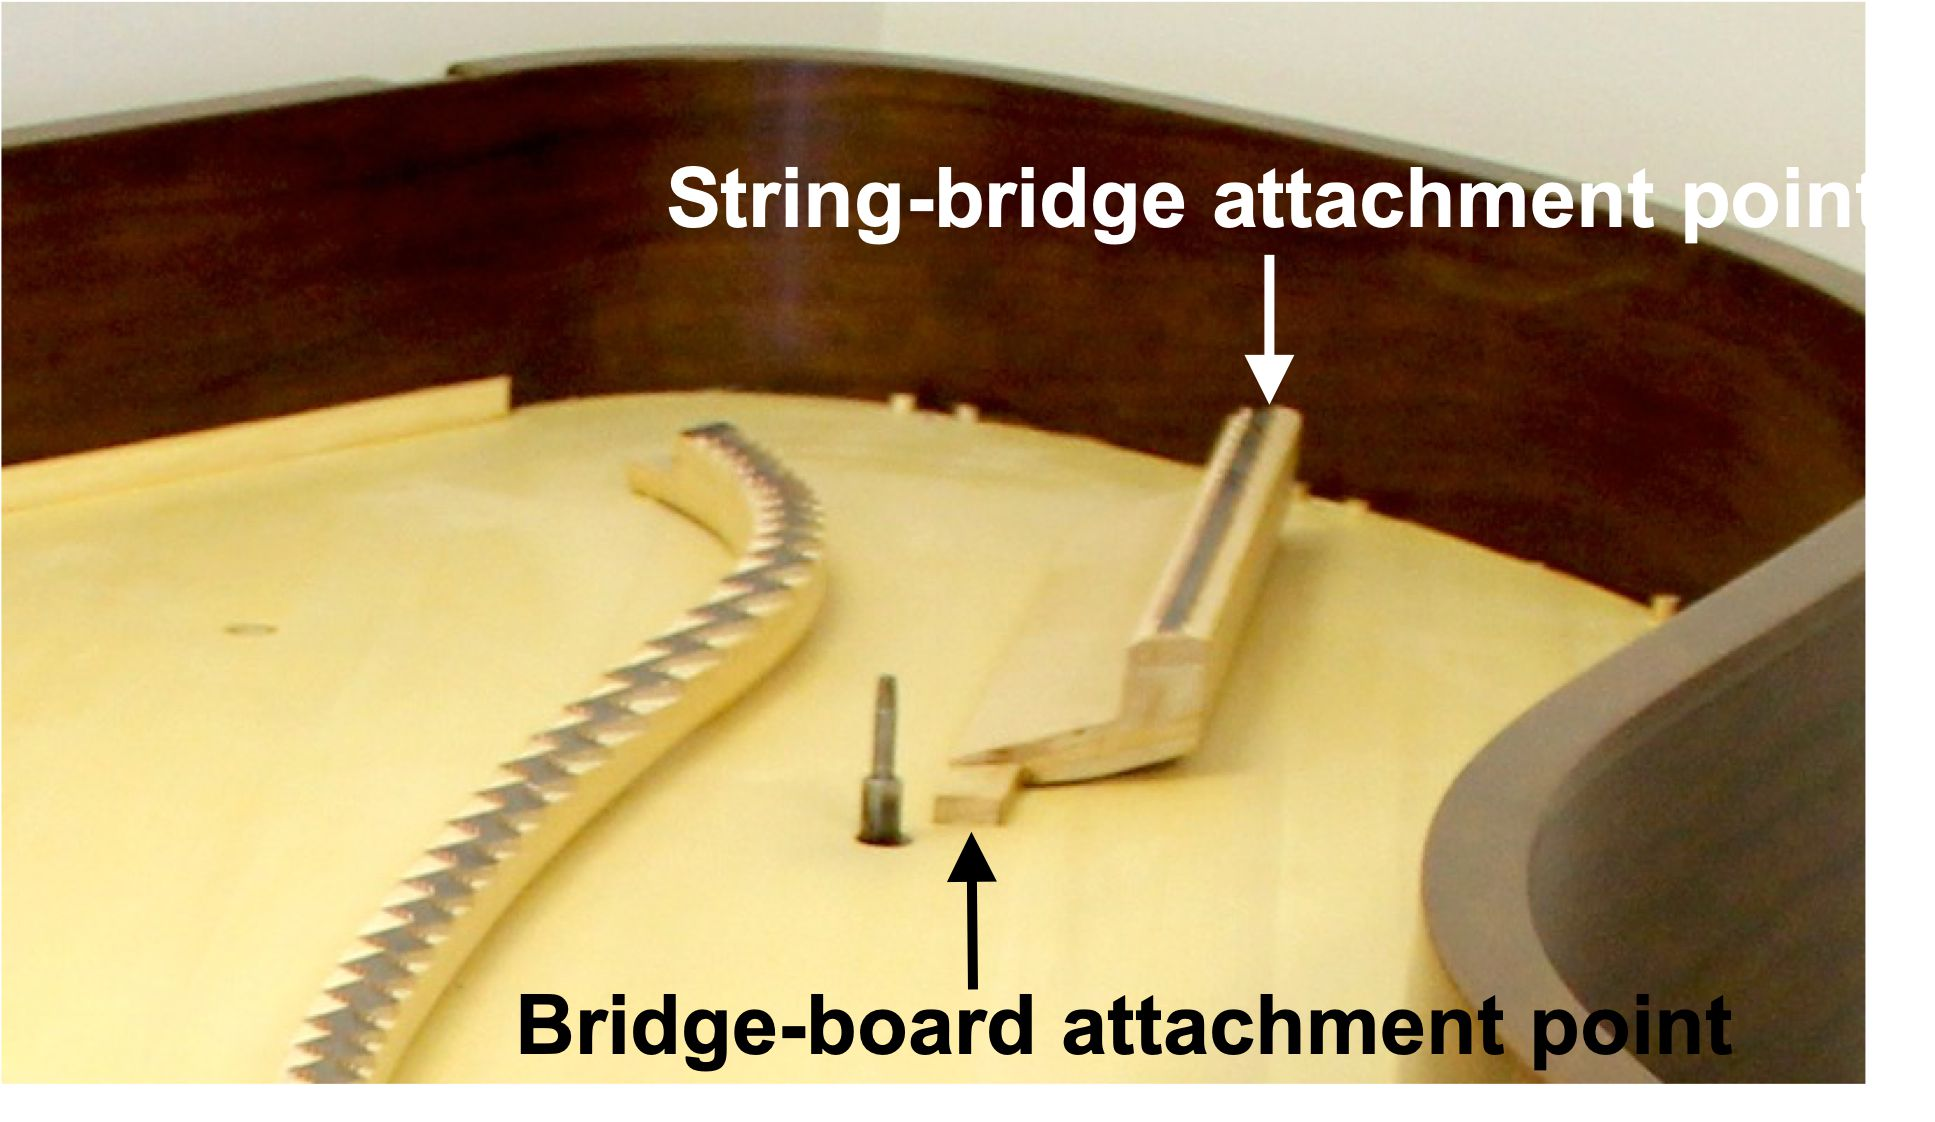
\includegraphics[width=0.7\linewidth]{00_Images/02_chapter/img256.jpg}
\caption{Cantilevered bridge concept for string-to-soundboard coupling}
\label{fig:cantilevered_bridges}
\end{figure}

\subsection{Sound Board}

For an upright piano, the soundboard can be idealized as a rectangular plate on which the treble and bass bridges are mounted. Trimming rims delimit the area effectively subject to vibration to an approximately trapezoidal region, while bridges run diagonally across it. This geometry is useful when comparing measurements performed on a simplified rectangular board without trimming rims. An upright soundboard and its simplified rectangular representation used for measurements are shown in figure \ref{fig:upright_soundboard_rectangular}.

\begin{figure}[!htb]
\centering
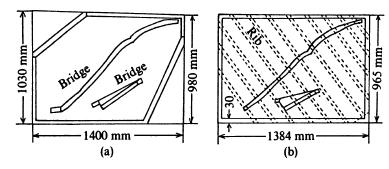
\includegraphics[width=0.7\linewidth]{00_Images/02_chapter/img271.jpg}
\caption{Upright soundboard and simplified rectangular representation for modal studies}
\label{fig:upright_soundboard_rectangular}
\end{figure}

Chladni figures measured on a rectangular soundboard illustrate the progression of mode shapes with frequency. Examples of Chladni patterns measured on a simplified soundboard are shown in figure \ref{fig:chladni_patterns_soundboard}.

\begin{figure}[!htb]
\centering
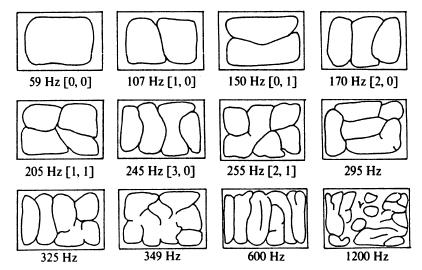
\includegraphics[width=0.7\linewidth]{00_Images/02_chapter/img285.jpg}
\caption{Chladni figures illustrating soundboard mode shapes}
\label{fig:chladni_patterns_soundboard}
\end{figure}

Low-order patterns can be associated with modal indices \( (m,n) \), for instance around
\[
\SI{59}{\hertz}\ (0,0), \quad \SI{107}{\hertz}\ (1,0), \quad \SI{150}{\hertz}\ (0,1), \quad \SI{170}{\hertz}\ (2,0), \quad \SI{205}{\hertz}\ (1,1)
\]
with increasingly complex nodal structures at higher frequencies, for example around \SI{600}{\hertz} and \SI{1200}{\hertz}. The observed modal frequencies lie between those expected for a board with clamped edges and a board with hinged edges. Since the bridge extends over a relevant fraction of the board length, the driving-point impedance measured on the bridge is expected to depend on the measurement location. A set of bridge points can be associated with the fundamental frequencies of the corresponding strings, spanning from low notes in the bass to very high notes in the treble. The measurement locations along the bridges, referenced to the corresponding string fundamentals, are shown in figure \ref{fig:bridge_measurement_points}. As a consequence, the mechanical impedance encountered by different string groups is not uniform along the bridge. Driving-point impedance measurements at different bridge locations show that minima of impedance often occur near the fundamental frequencies of the corresponding notes, which is a desirable feature for energy transfer and tonal balance. It is also observed that, above about \SI{1000}{\hertz}, the decrease of driving-point impedance is not particularly rapid in a grand piano. This behavior is often indicated as one reason for acoustic differences between grand and upright instruments. Radiation efficiency is strongly frequency dependent. Below the critical frequency of the soundboard, radiation efficiency drops because bending waves produce evanescent acoustic fields. Above a certain frequency, radiation resistance increases and can approach the characteristic impedance of air, although internal losses limit the effective radiation efficiency at high frequency. As a practical consequence, the frequency region that is favored for acoustic radiation is typically between \SI{200}{\hertz} and \SI{2000}{\hertz}. Driving-point impedance measured at different bridge locations is shown in figure \ref{fig:driving_point_impedance_locations}.

\begin{figure}[!htb]
\centering
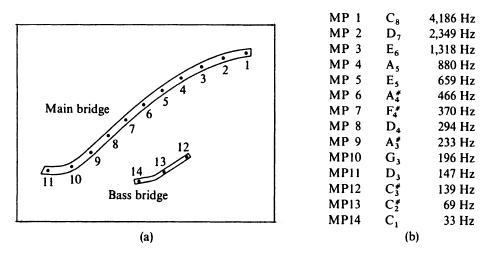
\includegraphics[width=0.65\linewidth]{00_Images/02_chapter/img299.jpg}
\caption{Bridge measurement points and corresponding string fundamental frequencies}
\label{fig:bridge_measurement_points}
\end{figure}

\begin{figure}[!htb]
\centering
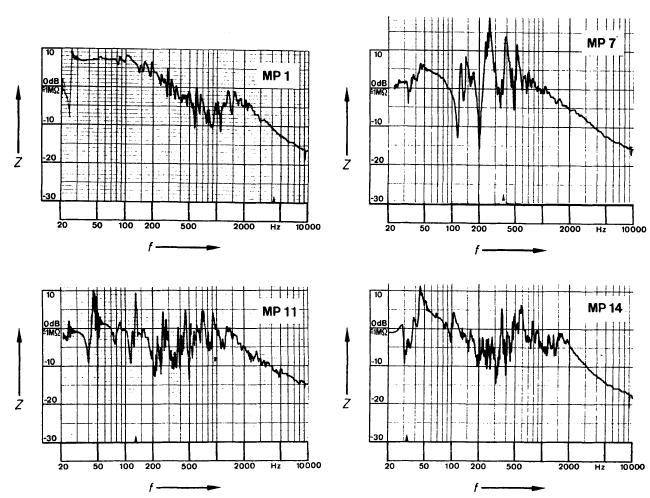
\includegraphics[width=0.65\linewidth]{00_Images/02_chapter/img313.jpg}
\caption{Driving-point impedance at different points along the bridge}
\label{fig:driving_point_impedance_locations}
\end{figure}

A comparison between the driving-point impedance and the radiated sound shows that impedance peaks do not always coincide with the dominant peaks in the radiated spectrum. One reason is that efficient radiation requires bending-wave speeds at those frequencies to be close to the speed of sound in air, which is satisfied only in a band near the critical frequency. Internal damping broadens this band and smooths the correspondence between mechanical peaks and radiated peaks. Overall radiation efficiency is affected by several factors, among which the position of the lid in a grand piano plays a relevant role. A representative comparison between mechanical impedance trends and radiated sound is shown in figure \ref{fig:impedance_vs_radiation}.

\begin{figure}[!htb]
\centering
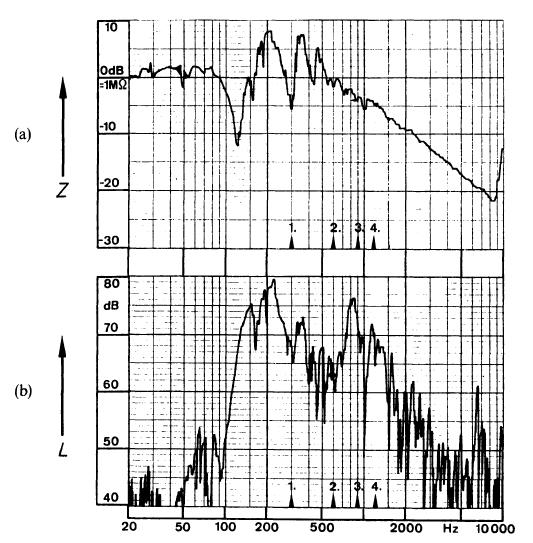
\includegraphics[width=0.6\linewidth]{00_Images/02_chapter/img329.jpg}
\caption{Comparison between driving-point impedance behavior and radiated sound level trends}
\label{fig:impedance_vs_radiation}
\end{figure}

Radiation patterns in a vertical plane show increased radiation over a range of angles when the lid is open. At low frequency it is desirable to increase bending-wave speed to improve radiation efficiency. This is attained by stiffening the board through ribs, while keeping the corresponding mass increase as small as possible. Since rib stiffness increases approximately with the square of rib height while rib mass is approximately proportional to height, a practical guideline is to use ribs that are narrow and high. Measured radiation patterns for different registers and lid configurations are shown in figure \ref{fig:radiation_patterns_lid_register}.

\begin{figure}[!htb]
\centering
\subfloat{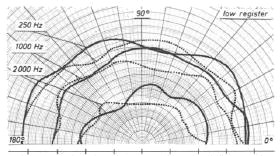
\includegraphics[width=0.3\linewidth]{00_Images/02_chapter/img349_1.jpg}}\hfill
\subfloat{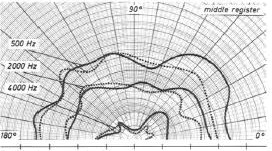
\includegraphics[width=0.3\linewidth]{00_Images/02_chapter/img349_2.jpg}}\hfill
\subfloat{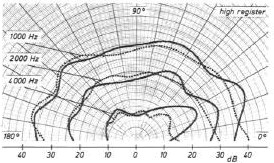
\includegraphics[width=0.3\linewidth]{00_Images/02_chapter/img349_3.jpg}}
\caption{Radiation patterns for different registers with lid open and closed}
\label{fig:radiation_patterns_lid_register}
\end{figure}

Sound levels across the full keyboard depend on playing force and illustrate that the radiated output varies substantially with register and excitation strength. The vibrational and radiative properties of a grand piano are markedly different from those of other piano types, particularly at low frequency. Overall sound levels across the full keyboard for different playing forces are shown in figure \ref{fig:sound_levels_88_notes}.

\begin{figure}[!htb]
\centering
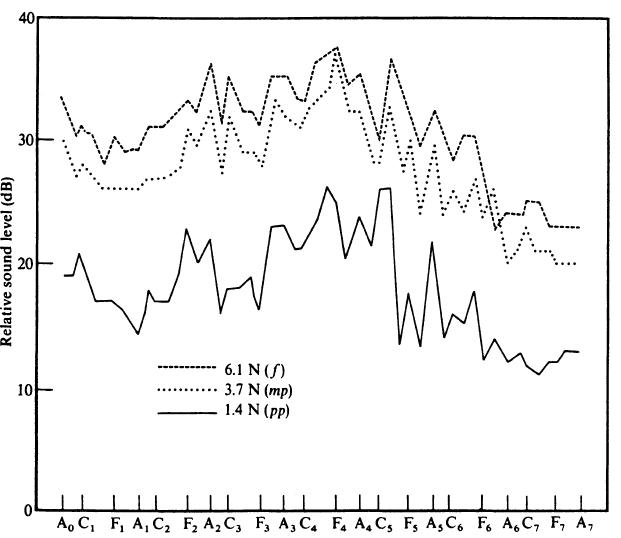
\includegraphics[width=0.55\linewidth]{00_Images/02_chapter/img367.jpg}
\caption{Sound levels across the 88 keys for different playing forces}
\label{fig:sound_levels_88_notes}
\end{figure}

Frequency responses obtained by exciting the soundboard at multiple points show that a small number of low-frequency modal peaks are consistently present in the measured spectra, and corresponding mode shapes can be identified. In addition, radiation efficiency can be large at several frequencies that are not at or near structural resonances. Two mechanisms are highlighted: cancellation of sound from different vibrating areas of the soundboard surface, and large volume velocity arising when two modes interfere strongly. Finally, when strings are mounted, the mobility (velocity/force) normal to the soundboard at bridge termination points decreases by about \SIrange{10}{15}{\decibel}. This is attributed to the high tension introduced by the strings, which limits soundboard mobility in the normal direction. A representative set of soundboard response spectra is shown in figure \ref{fig:soundboard_frequency_response}. Modal peaks and the link to corresponding mode shapes are summarized in figure \ref{fig:modal_peaks_mode_shapes}. Examples of soundboard mode shapes are shown in figure \ref{fig:soundboard_mode_shapes_1}. Additional mode-shape examples are shown in figure \ref{fig:soundboard_mode_shapes_2}.

\begin{figure}[!htb]
\centering
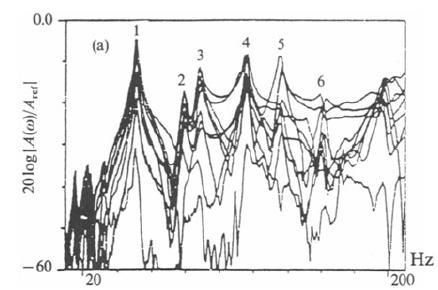
\includegraphics[width=0.55\linewidth]{00_Images/02_chapter/img381.jpg}
\caption{Soundboard frequency response showing multiple spectra overlaid}
\label{fig:soundboard_frequency_response}
\end{figure}

\begin{figure}[!htb]
\centering
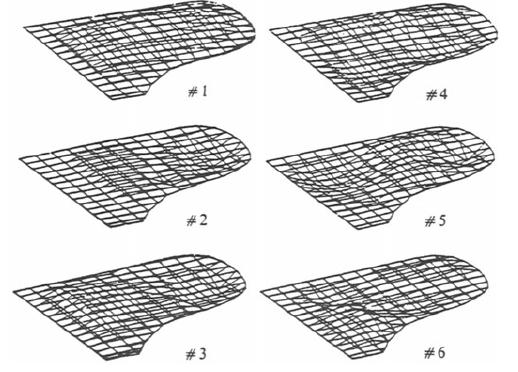
\includegraphics[height=0.27\textheight]{00_Images/02_chapter/img395.jpg}
\caption{Modal peaks in the response and corresponding mode-shape indications}
\label{fig:modal_peaks_mode_shapes}
\end{figure}

\begin{figure}[!htb]
\centering
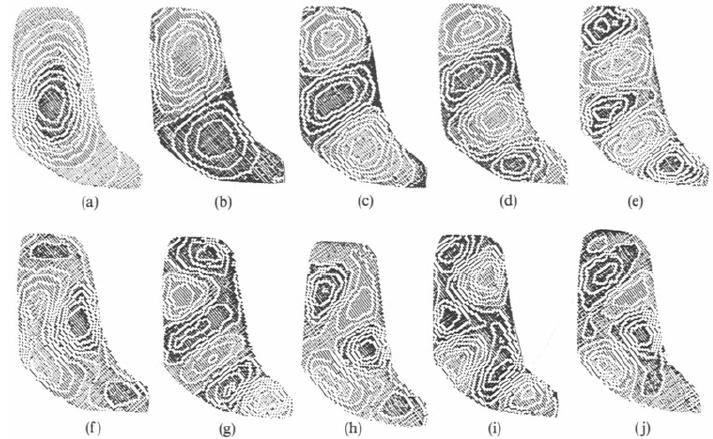
\includegraphics[height=0.27\textheight]{00_Images/02_chapter/img409.jpg}
\caption{Examples of soundboard mode shapes at selected resonant frequencies}
\label{fig:soundboard_mode_shapes_1}
\end{figure}

\begin{figure}[!htb]
\centering
\subfloat{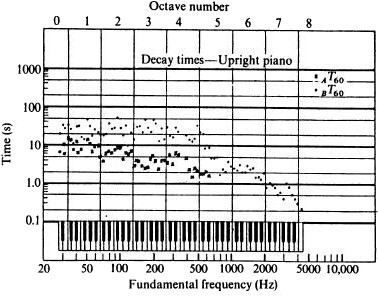
\includegraphics[width=0.45\linewidth]{00_Images/02_chapter/img435_1.jpg}}\hfill
\subfloat{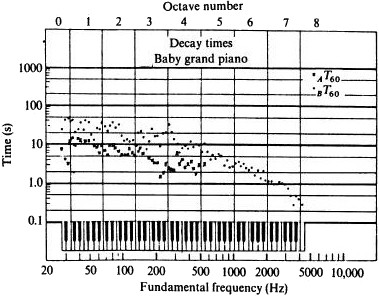
\includegraphics[width=0.45\linewidth]{00_Images/02_chapter/img435_2.jpg}}
\caption{Additional soundboard mode shapes illustrating the modal family over frequency}
\label{fig:soundboard_mode_shapes_2}
\end{figure}

\section{Sound Decay}

\subsection{Compound Decay and Decay Times}

The envelope of a piano tone typically exhibits a compound decay: an initial portion with a relatively high decay rate, followed by a second portion with a slower decay. Two phenomena are mainly responsible for this behavior: the change of polarization of the string motion during vibration and the coupling among strings within an unison group. To describe the decay in a compact way, two time measures are introduced:

\begin{itemize}
    \item \( AT_{60} \) is the reverberation time that would be observed if the faster initial decay continued unchanged.
    \item \( BT_{60} \) is the decay time associated with the overall tone, including the slower second part.
\end{itemize}

An example of compound decay and the definition of decay-time descriptors is shown in figure \ref{fig:compound_decay_AT_BT}.

\begin{figure}[!htb]
\centering
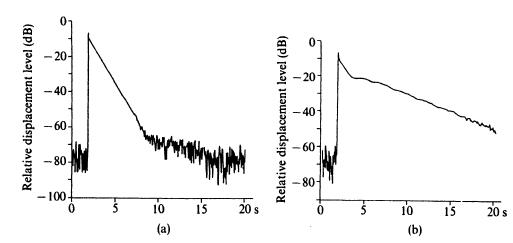
\includegraphics[width=0.7\linewidth]{00_Images/02_chapter/img454.jpg}
\caption{Compound decay and definition of \(AT_{60}\) and \(BT_{60}\)}
\label{fig:compound_decay_AT_BT}
\end{figure}

\subsection{Polarization-dependent Coupling to the Soundboard}

The soundboard impedance is not the same for different directions of string motion at the bridge. In particular, the impedance encountered for horizontal vibration is greater than for vertical vibration, because the soundboard is typically stiffer to tangential displacement than to orthogonal displacement. This difference can be observed by comparing decay curves measured on a single string, for instance for a \( D \sharp 4 \) string with fundamental frequency \( f=\SI{311}{\hertz} \), where the decay is markedly different for perpendicular and parallel polarizations. Polarization-dependent decay behavior for a representative note is shown in figure \ref{fig:polarization_dependent_decay}.

\begin{figure}[!htb]
\centering
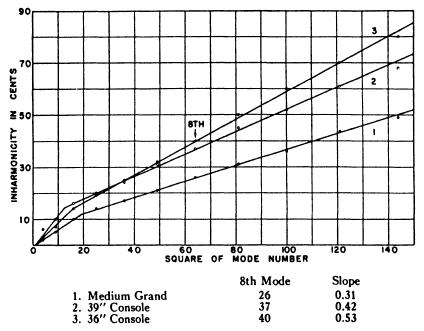
\includegraphics[width=0.6\linewidth]{00_Images/02_chapter/img469.jpg}
\caption{Decay curves for perpendicular and parallel polarizations of string motion}
\label{fig:polarization_dependent_decay}
\end{figure}

\subsection{Depolarization Mechanism During a Note}

When the hammer strikes the strings, the initial vibration polarization is mainly vertical. In the early stage of the note, the dominant impedance mismatch is therefore that between the string and the soundboard response to vertical displacement. For most strings, the spiral-like winding induces a net transfer of energy from the vertical polarization to the horizontal one. Since the vertical and horizontal displacements are out of phase, the motion can evolve toward a circular polarization. During the second part of the vibration, energy is then transmitted to the bridge also through the horizontal component. Because the mismatch between the string impedance and the soundboard impedance is much greater for horizontal than for vertical displacements, the energy transfer rate becomes smaller as the motion depolarizes. As a result, the tone tends to start with a rapid decay and then slow down over time.

\subsection{Unison Coupling and Phase Dispersion}

In unison groups, when the hammer strikes, the strings start vibrating approximately in phase. They therefore transfer energy to the soundboard in phase, which increases the effective transfer rate and contributes to the faster initial decay. Due to small tuning differences, after a few vibration cycles the strings gradually get out of phase. The resulting reduction in coherent energy transfer decreases the decay rate, producing a longer-lasting second part of the note. This depolarization-related effect can also be exploited in tuning practice to influence the perceived length of the aftersound.

\section{Tuning and Inharmonicity}

\subsection{Octave Stretching}

In a tuned piano, octaves are slightly stretched with respect to the ideal \( 2:1 \) frequency ratio, so that the octave note is set a bit higher than \( 2f \). There are two main reasons for adopting this practice.

\paragraph{Inharmonicity and beat reduction} Because of string stiffness, partials are stretched upward with respect to integer multiples of the fundamental. As a consequence, if an exact \( 2:1 \) octave is enforced, upper partials of the lower note can fall close to prominent partials of the upper note and produce audible beating. A slight octave stretch reduces such beats by improving the coincidence between relevant partials across the octave. This effect is stronger for short strings, which tend to exhibit larger inharmonicity. For this reason, octave stretching is typically more pronounced in upright pianos than in grand pianos.

\paragraph{Psychoacoustic motivation} A second contribution is perceptual: when two notes are several octaves apart, listeners tend to judge them as being in tune when a certain amount of stretch is present. For example, if a melody is about two octaves higher than the accompaniment, a stretching on the order of a semitone may be needed for the interval to be perceived as correctly tuned.

\subsection{Comparison Across Different Pianos}

A comparison of inharmonicity expressed in cents shows that smaller instruments generally exhibit higher inharmonicity than larger ones. The reported plot of inharmonicity versus the square of the mode number displays steeper trends for console pianos than for a medium grand, consistent with the stronger stiffness effects expected for shorter strings.

